\documentclass[11pt, a4paper]{article}

\usepackage[margin=1in]{geometry}
\usepackage{graphicx}
\usepackage{amsmath, amssymb}
\usepackage{listings}
\usepackage{xcolor}
\usepackage{hyperref}
\usepackage{booktabs}
\usepackage{subcaption}
\usepackage{float}
\usepackage{fancyhdr}
\usepackage{enumitem}

\pagestyle{fancy}
\fancyhf{}
\fancyfoot[C]{\thepage}

\begin{document}

\fancypagestyle{no_hdr_border_rule}{
  \renewcommand{\headrulewidth}{0pt}
}
\thispagestyle{no_hdr_border_rule}

\begin{center}
    {\Large \textbf{Experiment 8 -- Report}} \\[0.2cm]
    {\large \textbf{Digital Systems and Microcontrollers (DSM)}} \\[0.1cm]
    {\normalsize International Institute of Information Technology, Hyderabad} \\[0.3cm]
\end{center}

\vspace{0.2cm}
\hrule
\vspace{0.4cm}

\noindent \textbf{Student Name 1:} \textbf{Manbir Singh Judge} \hfill \textbf{Roll Number:} \textbf{2026113005} \\
\noindent \textbf{Student Name 2:} Charishma Kandregula \hfill \textbf{Roll Number:} 2026112022 \\
\noindent \textbf{Table Number:} 16 \hfill \textbf{Lab Room Number:} N114 \\
\noindent \textbf{Date of Experiment:} 30/10/2026

\vspace{0.4cm}
\hrule
\vspace{0.5cm}

\vspace{1em}

\tableofcontents
\vspace{0.5cm}
\hrule
\vspace{0.8cm}

\newpage
\fancyhead[L]{Experiment -- Report}

\fancyhead[R]{Experiment 8}

\section{Aim}
To implement and verify the operation of a binary cell for RAM based on RS flip-flop.

\section{Components \& Equipment Required}
\begin{itemize}
    \item Digital Test Kit (DTK) -- including power supply, switches, indicator LED pairs and breadboard
    \item \textbf{ICs}:
    \begin{itemize}[label=$\circ$]
        \item 7404 -- Hex Inverter
        \item 7411 -- Triple 3-input NAND
        \item 7404 -- Quad 2-input OR
    \end{itemize}
    \item Connecting Wires
\end{itemize}

\section{Circuit Diagram}
\begin{figure}[H]
    \centering
    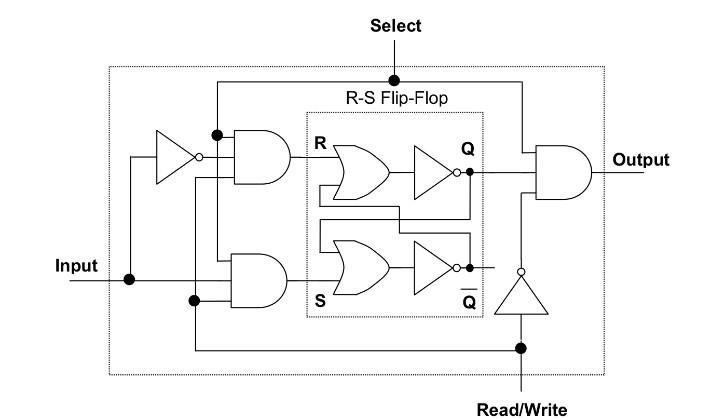
\includegraphics[width=0.75\textwidth]{ckt.png}
    \caption{Circuit Diagram for Circuit Diagram}
\end{figure}

\section{Procedure}
\begin{itemize}
    \item Place the required ICs on the breadboard and verify the operation of each gate.
    \item Wire the circuit according to the circuit diagrams using gates from above ICs.
    \item Apply all combinations of inputs and observe the results. Verify that observations match the expectation.
\end{itemize}

\section{Observations}
\begin{table}[H]
    \centering
    \begin{tabular}{|c|c|c|c|}
        \hline
        $S$ & $R/W$ & Operation & Output \\
        \hline
        0 & X & None & 0 \\
        \hline
        1 & 0 & Read & Q \\
        \hline
        1 & 1 & Write & 0 \\
        \hline
    \end{tabular}
\end{table}

Some observations:
\begin{itemize}
    \item During read operation, data input has no effect on $Q$.
    \item During write operation, output is set it to 0 and $Q$ is set to data input.
\end{itemize}

\section{Tinkercad Simulation}
\noindent \textbf{Tinkercad Link:} \href{https://www.tinkercad.com/things/iyuNRM4aOX3-dsm-experiment-8?sharecode=5GJvVXuBu0GV6i13xveY1A8NwDDoMIkECfBwB5GaE3s}{\color{blue}Click here}
\begin{figure}[H]
\centering
    \centering
    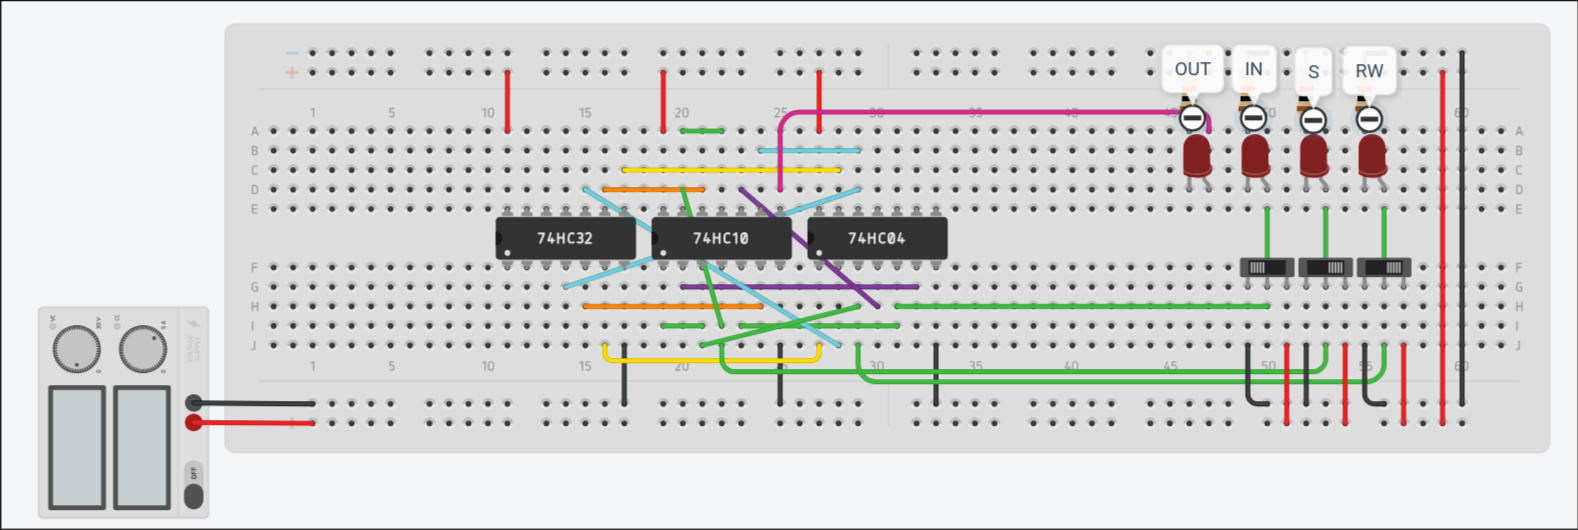
\includegraphics[width=\textwidth]{tc.png}
    \caption{Tinkercad Simulation Screenshot}
\end{figure}

\section{Hardware Setup Photograph}
\begin{figure}[H]
    \centering
    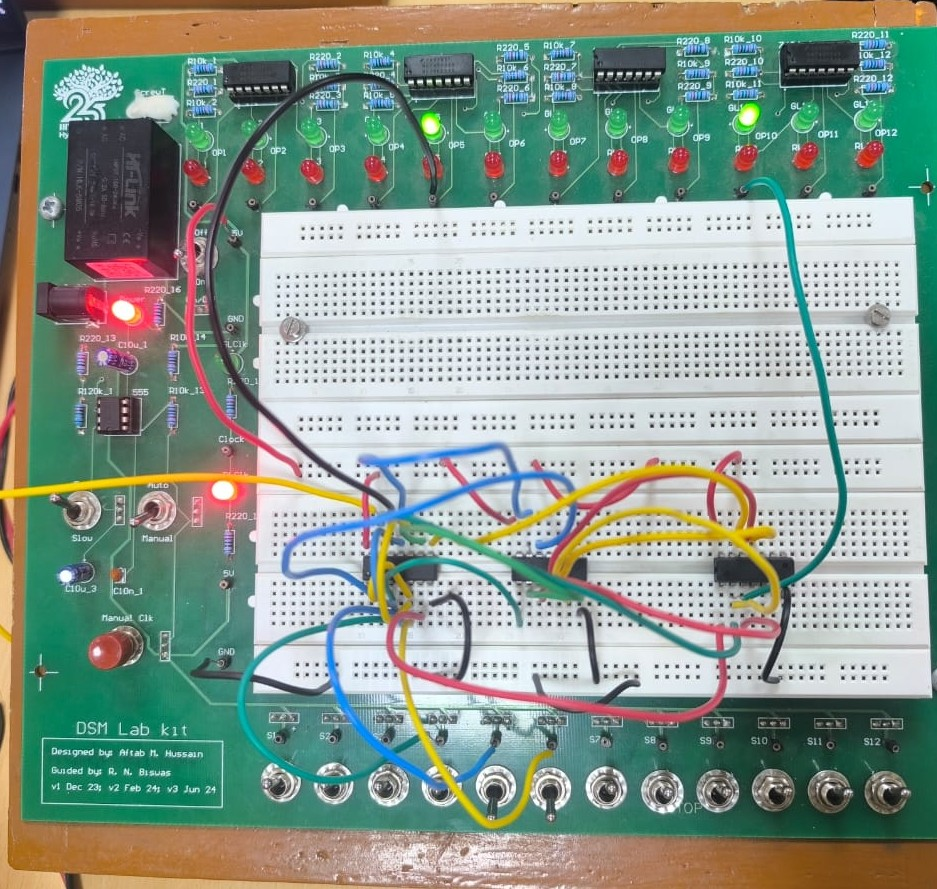
\includegraphics[width=0.75\textwidth]{lab.jpeg}
    \caption{Hardware Circuit for Serial Adder}
\end{figure}

\section{Conclusion}
A binary cell for RAM was implemented and its operation verified.

\end{document}